\section{Forecasts}

\subsection{Optimising Design Variables}

In a world where time and money are both finite, it is essential that we plan our experiments carefully and know what results we can expect from them. Since PMF detection is not the primary goal of future CMB experiments, it is useful to know before carrying out the analysis whether they have a chance to detect PMFs. Additionally, if the case ever arises that an experiment is designed for the sole purpose of detecting the signatures of PMFs in the CMB, we'd like to know how best to design that experiment. 

In order to find the best experimental set up and quantify the improvement from current constraints to future constraints, I used the mock covariances as described in section 3.3. I looked at 6 different experimental variables: Survey area, detector noise, beam width, $\ell_{knee}$, beam uncertainty and calibration uncertainty. For a full description of these variables refer to section 3.3. By varying one experimental variable at a time and holding the rest fixed, I was able to forecast the minimum experimental uncertainty on the PMF strength, $\sigma(B_{1Mpc})$ for each mock experiment and plot the relationship between $\sigma(B_{1Mpc})$ and the experimental variables.

\begin{table}[h]
\centering
\caption{Fixed Variables}
\label{table: fixed-stats}
\begin{tabular}{l|l}
\multicolumn{1}{c}{Variable} & \multicolumn{1}{|c}{Value} \\ \hline
\multicolumn{1}{c}{Survey area $(deg^2)$} & \multicolumn{1}{|c}{10313}  \\
\multicolumn{1}{c}{Noise ($\mu$K arcmin)} & \multicolumn{1}{|c}{1.9}   \\
\multicolumn{1}{c}{$\ell_{knee}$} & \multicolumn{1}{|c}{100} \\
\multicolumn{1}{c}{beam width (arcmin)} & \multicolumn{1}{|c}{4.0}   \\
\multicolumn{1}{c}{calibration error (\% error)} & \multicolumn{1}{|c}{0.01} \\
\multicolumn{1}{c}{beam uncertainty (\% error)} & \multicolumn{1}{|c}{0.05}
\end{tabular}
\begin{flushleft}
This table shows the values I chose for each independent variable when they were held fixed. The variables shown are all generous estimates for the range of capabilities the stage-3 experiments will have, but very conservative for stage-4. As a result, the forecasts will underestimate the strengths for the best-case scenario stage-4 experiments.
\end{flushleft}
\end{table}

\begin{figure}[h]
\centering
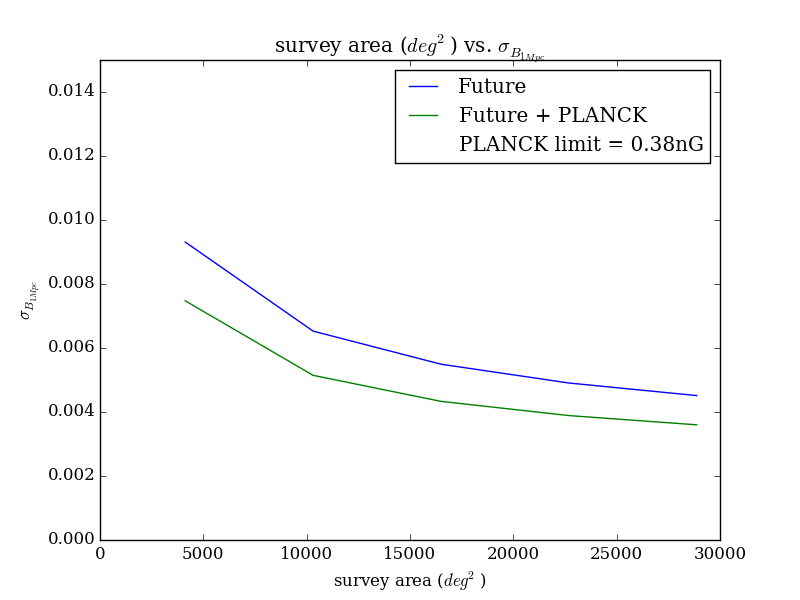
\includegraphics[scale=0.7]{images/area.png}
\caption{Increasing the survey area of future CMB experiments will return the best constraints on the value of $B_{1Mpc}$. This is a plot of survey area vs the uncertainty on $B_{1Mpc}$ with all other independent experimental variables held fixed. The blue line shows the precision for Future CMB experiments on their own and the green line shows the same precisions when combined with the Planck data set. Increasing survey area from 4,125 deg$^2$ to 28,877 deg$^2$ yields an improvement by roughly a factor of two. For reference, the current constraint is $\sigma(B_{1Mpc}) = 0.38nG$.}
\label{fig:area}
\end{figure}

\begin{figure}[h]
\centering
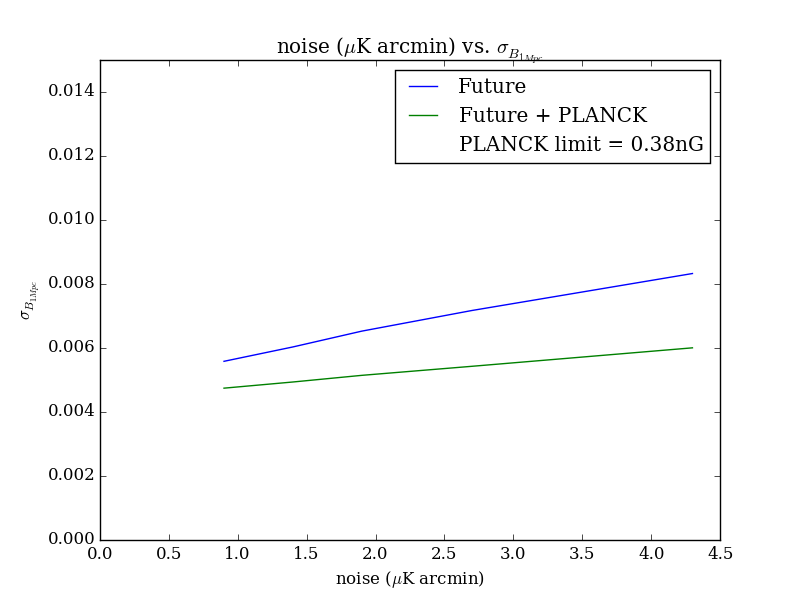
\includegraphics[scale=0.7]{images/noise.png}
\caption{The PMF constraints are still noise limited rather than cosmic variance limited. This is a plot of noise vs the predicted uncertainty on $B_{1Mpc}$. The blue line shows the predicted limits on $\sigma(B_{1Mpc})$ from future CMB experiments and the green line shows the predicted limits on $\sigma(B_{1Mpc})$ for future experiments combined with current Planck constraints. The minimum noise of 0.9$\mu$K arcmin corresponds with a detector count of $\sim$500,000 detectors. At this noise level $\sigma(B_{1Mpc}) \geq 0.0048nG$. This is a significant increase in precision over the current Planck limit, $\sigma(B_{1Mpc}) = 0.38nG$.}
\label{fig:noise}
\end{figure}

\begin{figure}[h]
\centering
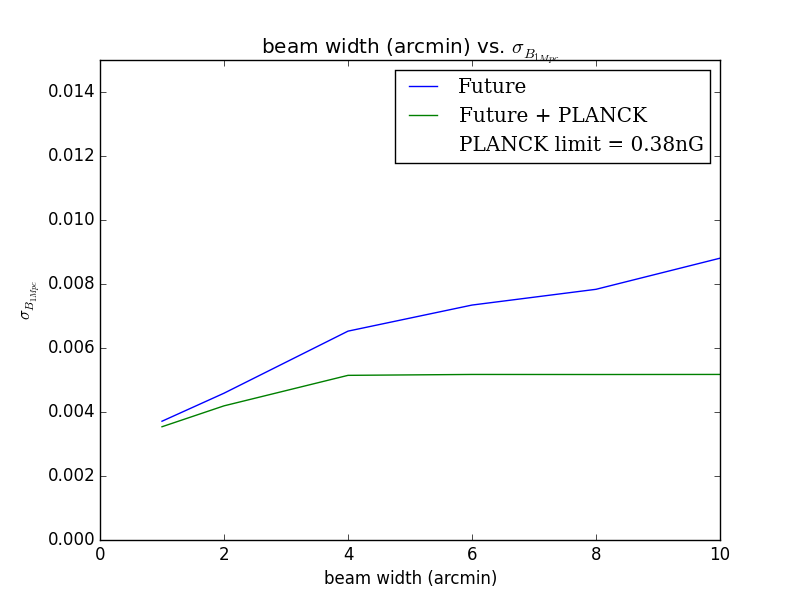
\includegraphics[scale=0.7]{images/width.png}
\caption{Reducing the the width of the beam, achieved by increasing the size of the telescope, reduces $\sigma(B_{1Mpc})$. This is a plot of beam width vs the uncertainty on $B_{1Mpc}$. The blue line shows the best constraints for $B_{1Mpc}$ for future CMB experiments and the green like shows the best constraints for $B_{1Mpc}$ for future CMB experiments plus Planck's constraints. The peak sensitivity for a beam width of 1 arcmin is $\sigma(B_{1Mpc}) \geq 0.0035nG$. This constraint is a major improvement over current Planck limits of $\sigma(B_{1Mpc}) = 0.38nG$.}
\label{fig:width}
\end{figure}

\begin{figure}[h]
\centering
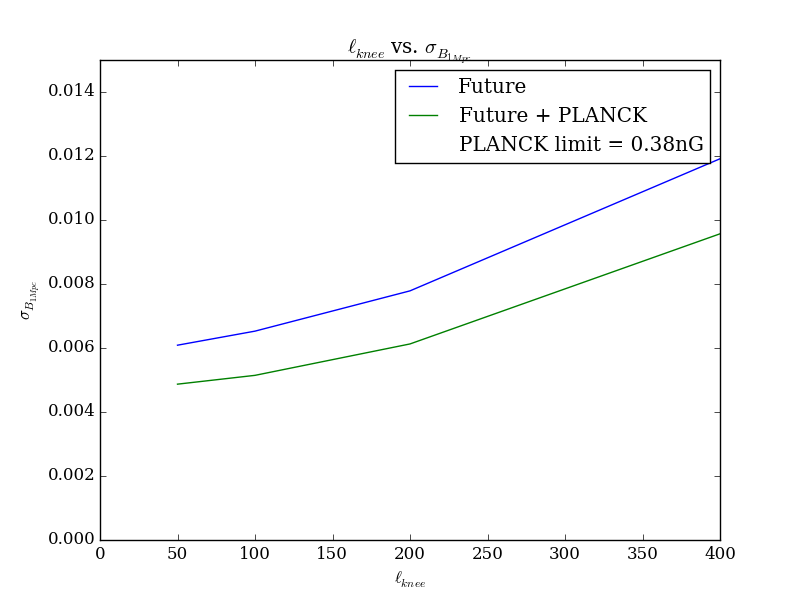
\includegraphics[scale=0.7]{images/knee.png}
\caption{Reducing $\ell_{knee}$ and hence increasing the stability of the experiment, also reduces $\sigma(B_{1Mpc})$. This is a plot of uncertainty on $B_{1Mpc}$ with all other variables held fixed. The blue line shows the best possible $\sigma(B_{1Mpc})$ for future experiments and the green line shows the best constraints for $\sigma(B_{1Mpc})$ for future experiments combined with prior limits from Planck. For $\ell_{knee} = 400$ we find the best constraint is $\sigma(B_{1Mpc}) \geq 0.0096$nG and for $\ell_{knee} = 50$ we find the best constraint is $\sigma(B_{1Mpc}) \geq 0.0049$nG. stage-3 and stage-4 shows a vast improvement over Planck's present limit of $\sigma(B_{1Mpc}) = 0.38nG$}
\label{fig:knee}
\end{figure}

Table ~\ref{table: fixed-stats} shows the fixed values for each experimental variable. The values match closest to the design specifications of the upcoming Simon's Observatory, which will see first light in 2019. The survey area is 10,313 square degrees, about a quarter of the full sky. The noise level is at 1.9$\mu$K arcmin corresponding to a detector count of $\sim$50,000. $\ell_{knee} = 100$ is adopted with a beam width of 4 arcmin. In addition, Calibration error and beam uncertainty are set to 0.01\% and 0.05\% respectively.

Since these values match the Simon's Observatory values, rather than the stage-4's specifications, the constraints on $\sigma(B_{1Mpc})$ will underestimate how well stage-4 will do. However, the trends we see in figures ~\ref{fig:area} to ~\ref{fig:knee} will still hold for a stage-4 experiment so whatever design choices benefit the Simon's Observatory will also benefit stage-4 experiments in the same way.

As expected, the optimal experimental design for detecting PMFs maximises the survey area and minimises noise. In addition beam width and $\ell_{knee}$ must also be minimised. The sensitivity is independent of the beam and calibration uncertainties.

As shown in figure ~\ref{fig:area}, $\sigma(B_{1Mpc})$ decreases as the survey area increases. If we combine the mock covariances with Planck data our best constraints range from $\sigma(B_{1Mpc}) \geq 0.0075nG$ for a survey area of 4,125 deg$^2$ to $\sigma(B_{1Mpc}) \geq 0.0036nG$ for a survey area of 28,877 deg$^2$, improving by a factor of 2.08. There is no controversy to say that experimentalists want to have an all-sky experiment however this can be impractical. 

While increasing the survey area gives better observations at large scales, it usually comes at the expense of good noise levels. Besides detector number, the depth of your scan can also impact noise levels. To reduce noise we'd like to take a scan that spends a long time per pixel, however our time is finite. If we spend too long scanning a pixel then our experiment can't scan a large area in a timely fashion. SPT-3G is one such experiment that trades survey area for depth, scanning an area of 2,500 square degrees. In contrast the Simon's Array scans a large area, of roughly 23,000 square degrees. Both return the same polarisation noise level if 4.8$\mu$K arcmin. A further problem with increasing the survey area is the galactic plane. The Milky Way galaxy blocks out light coming from the CMB and is a huge source of interference. As a result most experiments cut it out of their maps, trading away survey area for clearer signals.

Decreasing noise can yield up to a factor 1.28 improvement. At 4.3 $\mu$K arcmin we get $\sigma(B_{1Mpc}) \geq 0.0060nG$ and at 0.9 $\mu$K arcmin, $\sigma(B_{1Mpc}) \geq 0.0048nG$, as seen in figure ~\ref{fig:noise}. As discussed above noise isn't only gained from adding detectors, it also comes at the cost of survey area. However, if we do wish to add more detectors the obvious cost is grant money. It is rare that an experiment is fully funded, so often the number of detectors can't be as high as desired. Additionally fitting as many detectors into the experiment isn't always possible. There are size limitations. The number of detectors is limited by the size of the telescope and the size of each individual detector. As technology improves this ratio also does, but each experiment is usually representative of the technology available at the time and not of what is ideal.

As beam width decreases from 10 arcmin to 1 arcmin sensitivity improves by a factor of 1.46, reducing $\sigma(B_{1Mpc}) \geq 0.0052nG$ to $\sigma(B_{1Mpc}) \geq 0.0035nG$ as per figure ~\ref{fig:width}. Beam width is limited by how large we can build a telescope. If the telescope is too large, it becomes more expensive to build and maintain. In addition large telescopes become cumbersome and we may have to trade away some of our survey area to gain narrower beams.

In figure ~\ref{fig:knee}, we see that a lower $\ell_{knee}$ improves sensitivity. At $\ell_{knee} = 50$, $\sigma(B_{1Mpc}) \geq 0.0049nG$ and in the worst-case scenario, when $\ell_{knee} = 400$, we have $\sigma(B_{1Mpc}) \geq 0.0096nG$ - a factor of 1.96 improvement. $\ell_{knee}$ is a technical constraint. Ideally we'd like to have $\ell_{knee} = 0$ of course in practice this simply won't happen since we can never reduce noise to zero. The tradeoff here is between money and quality. A device with a low $\ell_{knee}$ will likely be expensive and a device with a high $\ell_{knee}$ will be cheaper. 

In contrast, changes to calibration and beam uncertainty have negligible effects on improving detection limits. For all values of beam and calibration uncertainties the sensitivity to the PMF strength is $\sigma(B_{1Mpc}) \geq 0.0051nG$.

The forecasts for the upcoming CMB experiments are promising. Our current best limits from Planck are $\sigma(B_{1Mpc}) = 0.38nG$. In comparison, the lowest limit from stage-3 and stage-4-like covariances are as low as $\sigma(B_{1Mpc}) = 0.0035nG$. In the most optimistic cases, measurements will have 100 times more sensitivity to PMFs than current experiments.

\subsection{Parameter Constraints}

Constraining the field strength of PMFs is not the only science goal of future CMB experiments. These experiments are also expected to constrain a wide variety of other model parameters characteristic of extensions to $\Lambda CDM$ cosmology. In this section I will provide the 1$\sigma$ confidence contours for $B_{1Mpc}$ and the selection of extended model parameters as described in Section 3.

By inverting Fisher matrices into covariance matrices, one can construct confidence ellipses for pairs of model parameters. The major and minor axes of the ellipse, $R_{major}$ and $R_{minor}$ are given by:

\begin{equation}
R_{major} = \sqrt{\frac{(\sigma_{xx} + \sigma_{yy})}{2} + \sqrt{\frac{(\sigma_{xx} - \sigma_{yy})^2}{4} + \sigma_{xy}^2}}
\end{equation}

\begin{equation}
R_{minor} = \sqrt{\frac{(\sigma_{xx} + \sigma_{yy})}{2} - \sqrt{\frac{(\sigma_{xx} - \sigma_{yy})^2}{4} + \sigma_{xy}^2}}
\end{equation}

where $\sigma{xy}$ are the covariances for the $x^{th}$ and $y^{th}$ model parameter. The angle of orientation of the confidence ellipse, $\theta$ is given by:

\begin{equation}
\theta = \frac{1}{2}arctan(\frac{2\sigma_{xy}}{\sigma_{xx}-\sigma_{yy}})
\end{equation}

For this analysis I took the Simon's Array as a typical stage-3 experiment as having a survey area of 10,313 square degrees, a noise level of 2.7$\mu$K arcmin and $\ell_{knee} = 100$. The typical stage-4 experiment improves on these variables with approximately two times the survey area, 22,689 square degrees, half the noise, at 1.3$\mu$K arcmin and $\ell_{knee} = 50$. Table ~\ref{table: stage-stats} shows the full set of 'typical' values I chose for the experimental variables of stage-3 and stage-4 experiments.

\begin{table}[h]
\centering
\caption{Mock Stage-3 and Stage-4 Variables}

\label{table: stage-stats}
\begin{tabular}{l|l|l}
\multicolumn{1}{c}{Variable} & \multicolumn{1}{|c}{Stage-3} & \multicolumn{1}{|c}{Stage-4} \\ \hline
\multicolumn{1}{c}{Survey area $(deg^2)$} & \multicolumn{1}{|c}{10313} & \multicolumn{1}{|c}{22689}  \\
\multicolumn{1}{c}{Noise ($\mu$K arcmin)} & \multicolumn{1}{|c}{2.7} & \multicolumn{1}{|c}{1.3}  \\
\multicolumn{1}{c}{$\ell_{knee}$} & \multicolumn{1}{|c}{100} & \multicolumn{1}{|c}{50} \\
\multicolumn{1}{c}{beam width (arcmin)} & \multicolumn{1}{|c}{4.0} & \multicolumn{1}{|c}{4.0}   \\
\multicolumn{1}{c}{calibration error (\% error)} & \multicolumn{1}{|c}{0.01} & \multicolumn{1}{|c}{0.01} \\
\multicolumn{1}{c}{beam uncertainty (\% error)} & \multicolumn{1}{|c}{0.05} & \multicolumn{1}{|c}{0.05}
\end{tabular}
\\
\begin{flushleft}
This table shows the values for each variable for both the mock covariance matrices used to construct the confidence ellipses. We see that from stage-3 to stage-4, the survey area will more than double from 10,313 square degrees to 22,689 square degrees, the noise will halve from 2.7$\mu$K arcmin to 1.3$\mu$K arcmin as will $\ell_{knee}$ - from 100 to 50. On the other hand, beam width will remains fixed at 4.0 arcmin and both beam and calibration errors stay at 0.05$\%$ and 0.01$\%$ respectively.
\end{flushleft}
\end{table}

As shown in figure ~\ref{fig:nrun}, stage-3 and stage-4 experiments make major improvements on $B_{1Mpc}$ and moderate improvements over $n_{run}$ from Planck results. The gains in precision in $n_{run}$ are significant from stage-3 to stage-4 in contrast to the gains in $B_{1Mpc}$. This relationship between $\sigma({B_{1Mpc})$ and $\sigma({n_{run})$ indicates that future CMB experiments will be effective for providing constraints on $n_{run}$. Additionally, There is a very weak degeneracy between the two parameters according to the Planck contour which seems to be broken by the contours from stage-3 and stage-4.

Figure ~\ref{fig:neff} shows that stage-3 and stage-4 experiments make moderate improvements on constraining $N_{eff}$ from current Planck results. The graph also shows that within Planck data there exists a degeneracy between the $B_{1Mpc}$ and the effective number of neutrinos. Stage-3 and stage-4 appear to break this degeneracy. Given the magnitude of the decrease in the size of the contours from Planck to stage-3 to stage-4, there is something to gain from using data from future CMB experiments to constrain $N_{eff}$.

Finally, figure ~\ref{fig:r} shows a drastic improvement on the constraints of $r$ from Planck to the next generations. This is to be expected since detecting primordial gravity waves from inflation is one of the primary science goals of ground-based CMB polarisation experiments. Data from stage-3 and stage-4 do not break the degeneracy that existed in Planck between $B_{1Mpc}$ and $r$ however. As a result, other methods for constraining the values of these parameters will be needed. The constraints for all the extended parameters and $B_{1Mpc}$ from Planck, stage-3 and stage-4 are shown in figure ~\ref{table: sigmas} 

\begin{table}[h]
\centering
\caption{Constraints for $\Lambda CDM$ Extensions}
\\
\label{table: sigmas}
\begin{tabular}{l|l|l|l}
\multicolumn{1}{c}{Variable} & \multicolumn{1}{|c}{Planck} & \multicolumn{1}{|c}{Stage-3} & \multicolumn{1}{|c}{Stage-4} \\ \hline
\multicolumn{1}{c}{$\sigma(B_{1Mpc})$} & \multicolumn{1}{|c}{0.244} & \multicolumn{1}{|c}{0.00627} & \multicolumn{1}{|c}{0.00373} \\
\multicolumn{1}{c}{$\sigma(n_{run})$} & \multicolumn{1}{|c}{0.00693} & \multicolumn{1}{|c}{0.00477} & \multicolumn{1}{|c}{0.00293} \\
\multicolumn{1}{c}{$\sigma(N_{eff})$} & \multicolumn{1}{|c}{0.200} & \multicolumn{1}{|c}{0.00536} & \multicolumn{1}{|c}{0.00329} \\
\multicolumn{1}{c}{$\sigma(r)$} & \multicolumn{1}{|c}{0.0531} & \multicolumn{1}{|c}{0.00169} & \multicolumn{1}{|c}{0.000622} \\
\end{tabular}
\\
\begin{flushleft}
This table shows the constraints on $\sigma(B_{1Mpc})$, $\sigma(n_{run})$, $\sigma(N_{eff})$ and $\sigma(r)$ from Planck, the Simon's Observatory and stage-4. All the constraints improve as the experiments improve. In $B_{1Mpc}$, $N_{eff}$ and $r$ we see a $\sim$100$\times$ improvement from current to stage-4 and in $n_{run}$ we see a $\sim$3$\times$ improvement
\end{flushleft}
\end{table}

\begin{figure}[h]
\centering
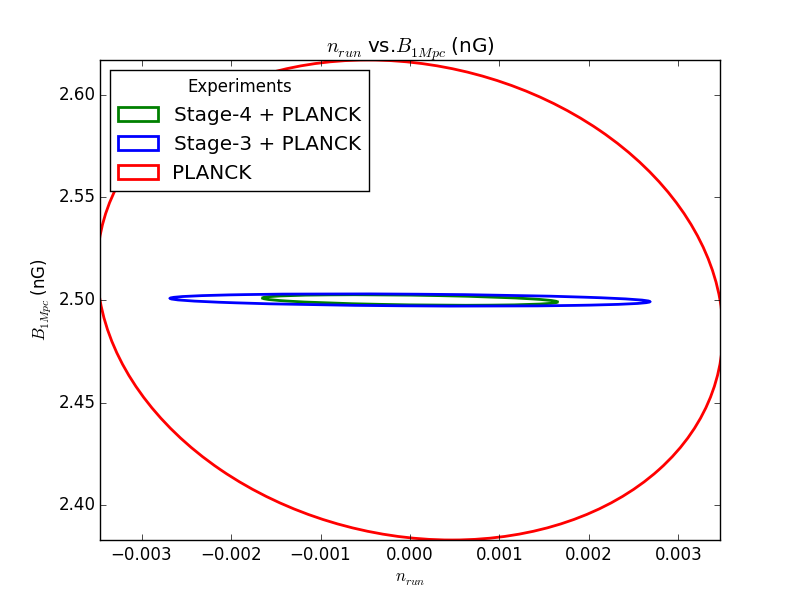
\includegraphics[scale=0.85]{images/contours/nrun.png}
\caption{Adding $n_{run}$ as an extension makes little difference to the PMF limits. This is a plot of the 1$\sigma$ confidence contours for $n_{run}$ vs. $B_{1Mpc}$. The red line shows the confidence contour for previous Planck data. The blue contour shows the confidence contour for stage-3 CMB experiments plus Planck data. The green contour shows the confidence contour for stage-4 CMB experiments plus Planck data. The plot shows a large forecasted improvement on the stage-3 and stage-4 precisions on $B_{1Mpc}$ over the previous Planck constraints. Improvements on $n_{run}$ increase from Planck, where $\sigma(n_{run}) =$ 0.00693 to stage-3 with $\sigma(n_{run}) =$ 0.00477 and finally to stage-4 with $\sigma(n_{run}) =$ 0.00373.}
\label{fig:nrun}
\end{figure}

\begin{figure}[h]
\centering
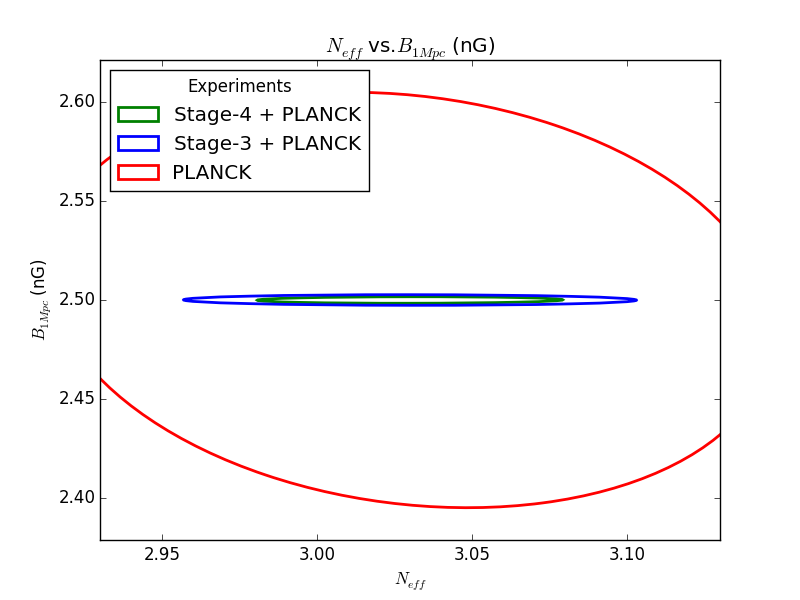
\includegraphics[scale=0.85]{images/contours/neff.png}
\caption{Marginalising over the number of relativistic species of neutrino, $N_{eff}$ does not weaken the PMF measurement. This is a plot of the 1$\sigma$ confidence contours for $N_{eff}$ vs. $B_{1Mpc}$. The red line shows the confidence contour for previous Planck data. The blue contour shows the confidence contour for stage-3 CMB experiments plus Planck data. The green contour shows the confidence contour for stage-4 CMB experiments plus Planck data. The plot shows moderate improvements on $\sigma(B_{1Mpc})$, with stage-4 experiments possessing the tightest constraints, as expected. Improvements on $N_{eff}$ increase from Planck, where $\sigma(N_{eff}) =$ 0.2 to stage-3 with $\sigma(N_{eff}) =$ 0.00536 and finally to stage-4 with $\sigma(N_{eff}) =$ 0.00329.}
\label{fig:neff}
\end{figure}

\begin{figure}[h]
\centering
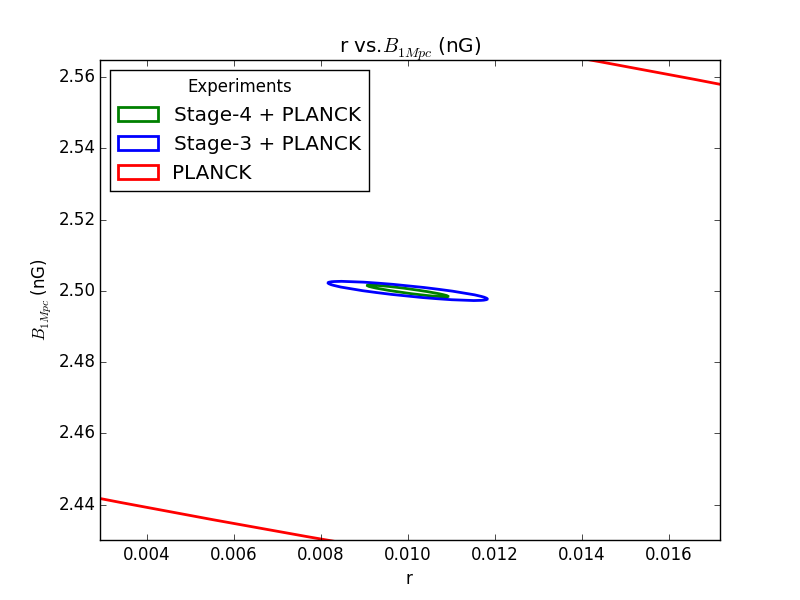
\includegraphics[scale=0.85]{images/contours/52.png}
\caption{This is a plot of the 1$\sigma$ contours for $r$ vs. $B_{1Mpc}$. The red line shows the confidence contour for previous Planck data. The blue contour shows the confidence contour for stage-3 CMB experiments plus Planck data. The green contour shows the confidence contour for stage-4 CMB experiments plus Planck data. There is a large forecasted improvement in both the constraints on $B_{1Mpc}$ and $r$ over previous Planck data, however neither stage-3 or stage-4 are expected to break the degeneracy between $B_{1Mpc}$ and $r$. Improvements on $r$ and $B_{1Mpc}$ increase from Planck, where $\sigma(r) =$ 0.0531 and $\sigma(B_{1Mpc}) =$ 0.244 and to stage-3 with $\sigma(r) =$ 0.00169 and $\sigma(B_{1Mpc}) =$ 0.00627 and finally to stage-4 with $\sigma(r) =$ 0.000622 and $\sigma(B_{1Mpc}) =$ 0.00373.}
\label{fig:r}
\end{figure}
